\documentclass[a4paper, 11pt]{article}
\usepackage{comment} 
\usepackage{fullpage}
\usepackage{amsmath} 
\usepackage{amssymb} 
\usepackage{mathtools}
\usepackage{siunitx}
\usepackage{xfrac}
\usepackage{icomma}
\usepackage[section,below]{placeins}
\usepackage[labelfont=bf,font=small,width=0.9\textwidth]{caption}
\usepackage{subcaption}
\usepackage{graphicx}
\usepackage{grffile}
\usepackage{float}
\floatplacement{figure}{htbp}
\floatplacement{table}{htbp}
\usepackage{booktabs}
\usepackage{hyperref}
\usepackage{pdfpages}
\sisetup{separate-uncertainty=true}

\begin{document}
\noindent
\centerline{\small{\textsc{Michigan State University}}} \\
\large{\textbf{CMSE 823 – Numerical Linear Algebra \hfill Spring 2020 \\
Homework 5}} \\
Alexander Harnisch \\
\noindent\makebox[\linewidth]{\rule{\textwidth}{0.4pt}}

\section*{1.}
We re-use the implementations from the previous homework, you can find them
again in the file \textit{qr.py}.

\section*{2.}
For solving the over and well-determined systems we can use Algorithm 11.2. For
under-determined systems we simply transpose the system which effectively
converts it into an over-determined system. Everything is pretty much the same.

So instead of $Ax=b$ we solve $x^\textup{T}A^\textup{T}=b^\textup{T}$ and
perform the reduced QR decomposition on $A^\textup{T}$ instead. Now we have the solution:
\begin{equation}
  x^\textup{T} = b^\textup{T}R^{-1}Q^{\textup{T}}
\end{equation}
or equivalently
\begin{equation}
  x = QR^{-\textup{T}}b = Qy
\end{equation}
where we find y by forward substitution, since 
\begin{equation}
  R^\textup{T}y = b
\end{equation}
with $R^\textup{T}$ being lower triangular.

I don't know how much of this is going to be discussed in class, I don't have
time to wait for it, it doesn't fit my schedule. I also could not find this
explicitly in the textbook.

You can find my implementation of the forward and backward substitution in
\textit{solve.py}. Note that for small $n$ it is actually faster to calculate
the inner product of $x$ and $r_j$ (or $l_j$ in the forward case) in each step
when $x$ has been initialized as a zero vector. I showed both ways to implement
it by implementing forward and backward subsection in those two different ways.

\subsection*{(a) (b) and (c)}
To get the results for the given matrices run \textit{hw05\_02.py}. As you can
see, the results are correct using all different methods for obtaining the QR
decomposition. The output should look as follows:

\begin{verbatim}
Part (a)
--------
Solving ax=b with a =
[[1 2 3]
 [4 5 6]
 [7 8 7]
 [4 2 3]
 [4 2 2]]
and b =
[ 6. 15. 22.  9.  8.]

Classical Gram-Schmidt: x =
[1. 1. 1.]

Modified Gram-Schmidt: x =
[1. 1. 1.]

Householder Method: x =
[1. 1. 1.]

Part (b)
--------
Solving ax=b with a =
[[0.7     0.70711]
 [0.70001 0.70711]]
and b =
[1.40711 1.40712]

Classical Gram-Schmidt: x =
[0.99999352 1.00000641]

Modified Gram-Schmidt: x =
[0.99999352 1.00000641]

Householder Method: x =
[1. 1.]

Part (c)
--------
Solving ax=b with a =
[[1 2 3]
 [4 2 9]]
and b =
[ 6 15]

Classical Gram-Schmidt: x =
[0.42857143 0.85714286 1.28571429]

Modified Gram-Schmidt: x =
[0.42857143 0.85714286 1.28571429]

Householder Method: x =
[0.42857143 0.85714286 1.28571429]
\end{verbatim}

\section*{3.}
\subsection*{(a) and (b)}
See the following handwritten page.
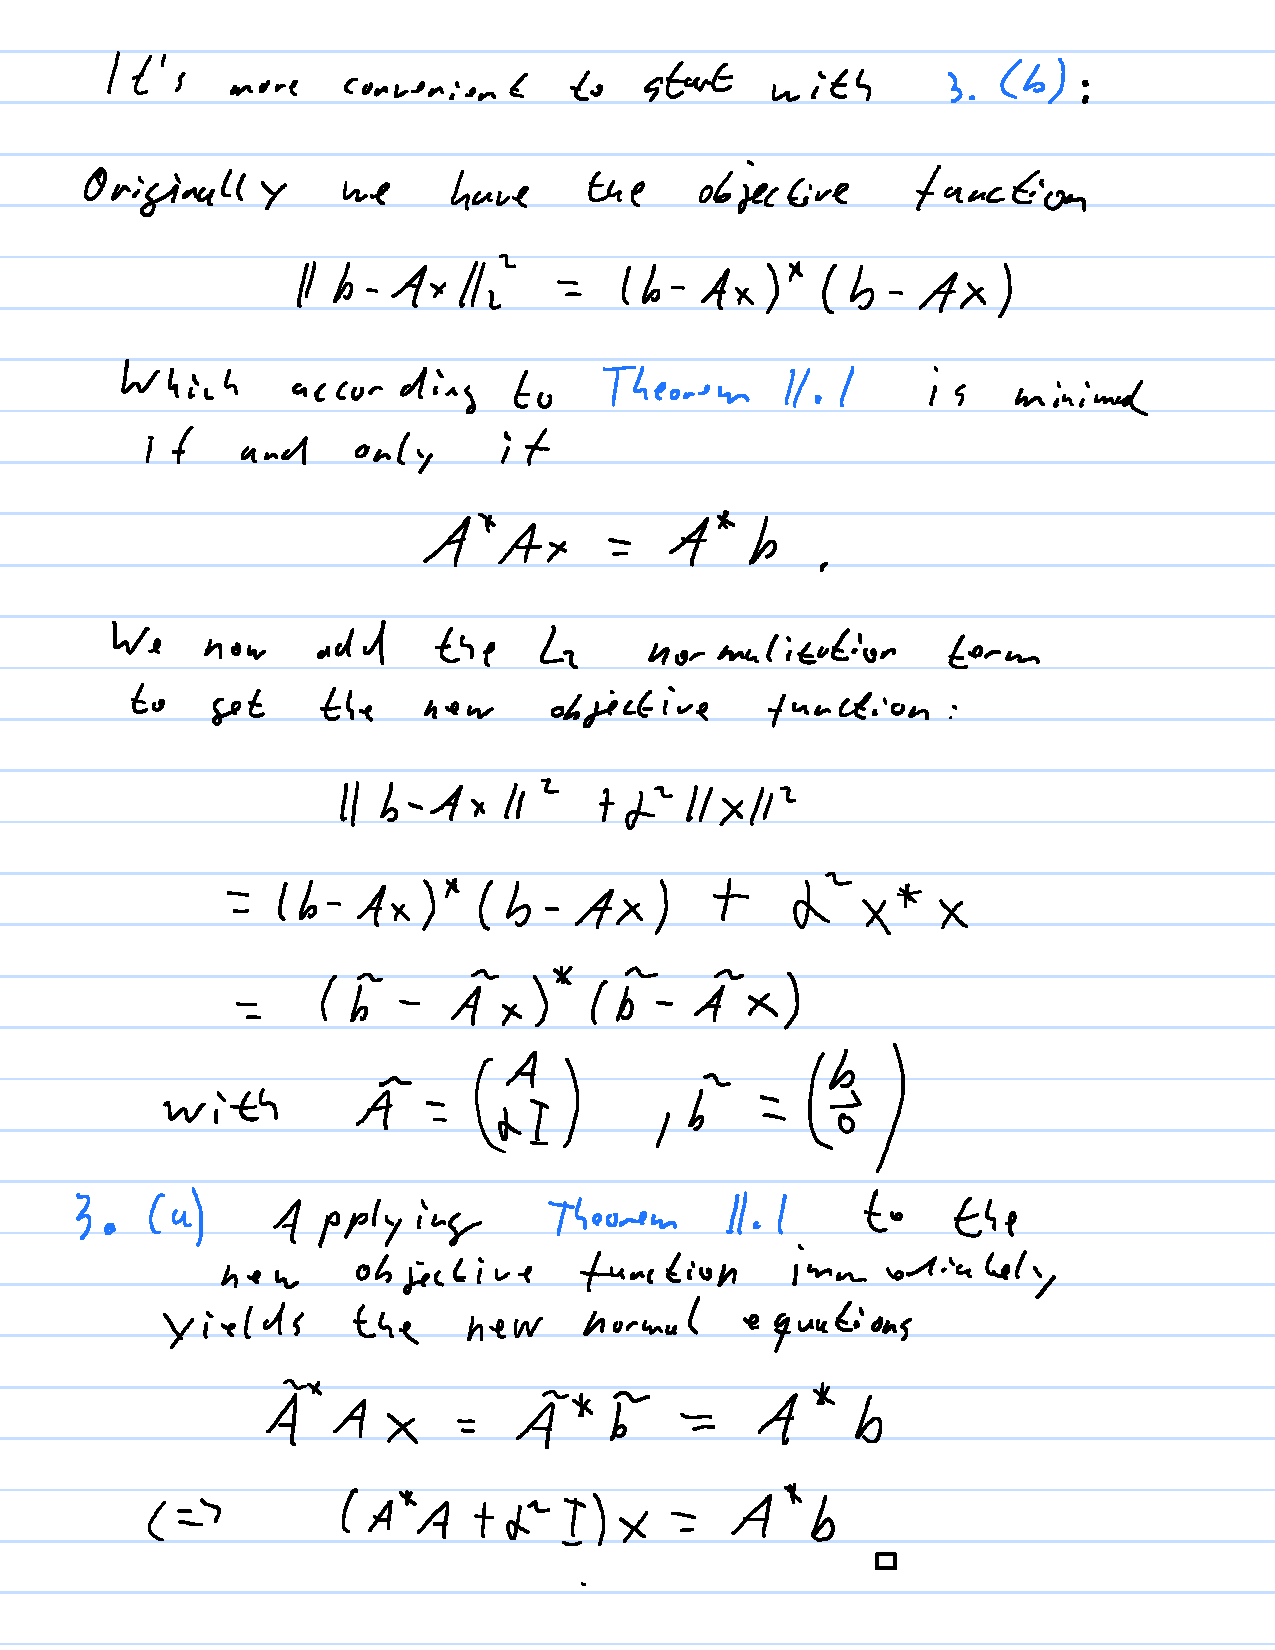
\includepdf{../3_a_b.pdf}

\newpage
\subsection*{(c)}
You can find the code in the file \textit{hilbert.py}.

\end{document}
